\documentclass{article}
\usepackage[utf8]{inputenc}
%\usepackage{natbib}
\usepackage{graphicx}
\usepackage[hidelinks]{hyperref}
\usepackage{color}
\usepackage{listings}
%\usepackage{lastpage}
%\usepackage{wrapfig}
%\usepackage{eso-pic}
%\usepackage{tikz}
\usepackage{float}
\usepackage{amssymb}
\usepackage{caption}
\usepackage{subcaption}
%\usepackage{pdfpages}
\usepackage[backend=biber]{biblatex}
\definecolor{commentgreen}{RGB}{100, 190, 100}
\definecolor{gray}{RGB}{50, 50, 50}
\lstset{language=C,
                breaklines=true,
                basicstyle=\ttfamily\scriptsize,
                keywordstyle=\color{blue}\ttfamily,
                stringstyle=\color{red}\ttfamily,
                commentstyle=\color{commentgreen}\ttfamily,
                morecomment=[l][\color{magenta}]{\#},
                numberstyle=\tiny\color{gray},
                numbers=left
}


\title{CGP - Mini-project:\\Water Shader}
\author{Jannick Drews}
\date{\today}

\newcommand{\secref}[1]{\nameref{#1}~\ref{#1}}
\newcommand{\goodcite}[1]{\textsuperscript{\cite{#1}}}

\addbibresource{Ref.bib}

\setlength\parindent{0pt}
\begin{document}
\pagenumbering{gobble}
\maketitle
\newpage
\pagenumbering{arabic}

%% For this mini-project, you have to create and showcase an advanced shader and talk about the theory behind it.
%% You should be able to depict a deep understanding of your code, to be able to explain how it works and how you
%%  overcome the technical challenges you met.  Such shader can be, but not limited to: %% list of suggestions here%%
%%

\section{Abstract}
\label{sec:abstract}
%what is the problem
Water shaders are finicky when it comes to realism. A water shader would be easy to implement, if it did not need reflections and refractions to come across realistic.\\
%what others have done
Usually the water shaders are made with a seamless normal map multiplied over a time variable. The shaders also includes refractions which must in addition to transforming the objects behind the mesh with the shader applied, visually in some arbitrary direction based on, usually, snells law.\\
%why its still a problem
We have come far with water shaders, you could even say that we have reached a good verdict on the realistic looks of it.
%what i propose
I chose to make a water shader with a voronoi bump map on the vertex level to create an artistic approach compared to making the standard convetional water shaders. This was to see if voronoi could make realistic waves compared to a static normal map.

\section{Introduction}
\label{sec:introduction}
A water shader can be built in many different ways, this report will cover how I developed my shader, the challenges I faced and how I reached my goals. To start with I was looking for a unique way to develop the water shader, usually the shader is made using a bump or normal map for the water itself, in this project I was aiming for using voronoi as the bump map.

\section{Theory}
\label{sec:theory}
This section will cover all theory related to the shader. This will include; Voronoi, bump maps, reflections and refractions, fragment and vertex knowledge, fresnel effect, transparency, culling, and grabpass.

\subsection{Fragment \& Vertex}
\label{sec:frag_vert}
The \textbf{fragment} and \textbf{vertex} shaders are both shaders but they work in different spaces. The vertex shader works on the local space, object space and afterwards converts the space to the clip space. The fragment shader works by modifying the mesh on the clip space, which will finally be convert to screen space\cite{progrendervertfrag}.


\subsection{Voronoi}
\label{sec:voronoi}
The voronoi effect is made by having, typically a grid of 9 cells which each have a random point, and from that point a distance is calculated to each other cell. Depending on that distance, each pixel will be colored with less and less saturation. You could argue that it is a radial colouration that happens, colouring outwards from the center point.\\

\begin{figure}[H]
    \centering
    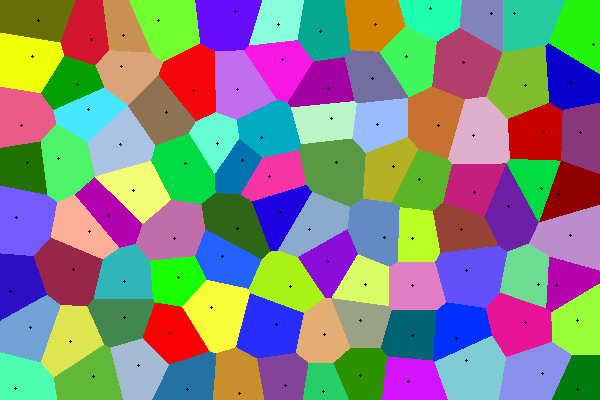
\includegraphics[width=.75\textwidth]{img/voronoi}
    \caption{Voronoi\protect\footnotemark}
    \label{fig:voronoi}
\end{figure}
\footnotetext{\url{https://www.codeproject.com/KB/recipes/882739/Fig_1.png}}
\autoref{fig:voronoi} shows the voronoi effect. Each cell is uniquely coloured to better showcase the effect, the voronoi effect is usually coupled with a time variable with a sinus or cosinus function applied to make each cell move with time passed.\\

I've used this effect on the vertex shader, applying it in object space as to generate a bump map which I utilize to visualize the waves on the object. The voronoi affect is applied via the normals of the mesh.
% UI scaling etc

\subsection{Bump maps}
\label{sec:bump_map}
Bump maps in shaders is utilized by having a greyscale image or texture tell where the object should modify the verteces positions. Ergo translating the position of the verteces to a new position after shader application. This can be applied to either the vertex or fragment shader respectively.

\begin{figure}[H]
    \centering
    \lstinputlisting[firstline=103, lastline=108]{img/voronoi.shader}
    \caption{Displacement - code implementation in object space}
    \label{fig:displacement}
\end{figure}
\autoref{fig:displacement} shows the code implementation for the bump map formula used to generate the shaders bump maps based on the voronoi greyscale.

\subsection{Reflections \& Refraction}
\label{sec:refl_refr}
%TODO reflections math, UNITYCG
The reflections are based on the camera position and aangle towards the object holding the shader.\\

Two vectors are needed to generate reflections based on the camera and object positions. Firstly, the vector from the camera to the object is calculate, then the normal vector gets calculated from the vertex normals. These two variables are then inserted into a \texttt{reflect} function which calculates the reflections needed.
\begin{figure}[H]
    \centering
    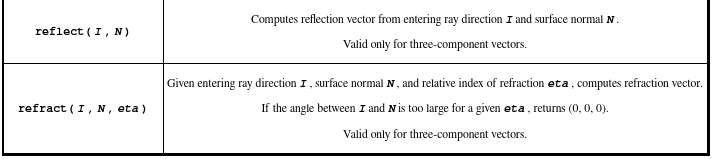
\includegraphics[width=\textwidth]{img/nvidia}
	\caption{Nvidia documentation - reflect \& refract}
    \label{fig:nvidia_refl_refr}
\end{figure}
\autoref{fig:nvidia_refl_refr} shows the documentation for the refract and reflection functions which Unity utilizes.
Snell's law:
$$ \eta_1 sin\theta_i = \eta_2 sin\theta_t $$
This formula describes the vector angle shift when entering another medium from a first.
\begin{figure}[H]
    \centering
	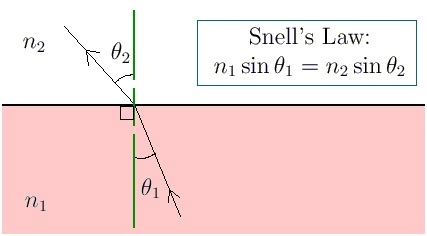
\includegraphics[width=.75\textwidth]{img/snell}
	\caption{Snell's law illustration\protect\footnotemark}
    \label{fig:snells_illustration}
\end{figure}
\footnotetext{\url{http://s3-ap-southeast-1.amazonaws.com/subscriber.images/physics/2016/10/28112355/Snells-Law.jpg}}
\autoref{fig:snells_illustration} shows how Snell's law would work with an example vector between two mediums. We can see that the vector changes direction based on the entering angle. Depending on the refraction index, the vector will then move in a new direction if the refraction indeces differs from eachother.

\subsubsection{Grabpass}
\label{sec:grabpass}
%TODO Grap-pass code from unity and EXPLAIN
\begin{figure}[H]
	\centering
	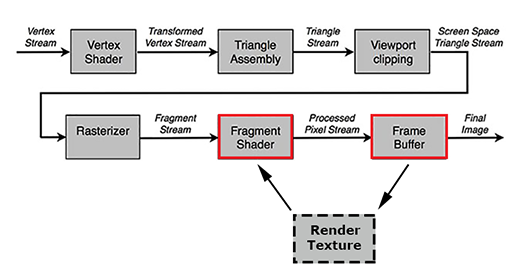
\includegraphics[width=\textwidth]{img/grabpass}
	\caption{Grabpass illustration}
	\label{fig:grabpass}
\end{figure}
\autoref{fig:grabpass} shows the illustration of how grabpass works. When the frame buffer is reached in the pipeline, it projects that buffer onto a render texture, so it kind of "grabs" the screen before it arrives at the final output. We can then modify this render texture however we want and use it for e.g. refractions.

\subsection{Fresnel effect}
\label{sec:fresnel_effect}
The Fresnel effect is blablabla..\\It can be used to visualize reflective objects color, when viewed at a critical angle. The effect is a bright surface, which will form around the object, no matter the camera angle, and is applied in clipspace.
%\begin{figure}[H]
%    \centering
%    \includegraphics[width=.75\textwidth]{img/fresnel}
%    \caption{Voronoi\protect\footnotemark}
%    \label{fig:voronoi}
%\end{figure}



% Voronoi
% Bump map
% Reflection & Refraction(distort)
% Additive color
% Local space & clip space
% Fragment & vertex shader
% Fresnel
% Transparency & the NON usage of it
% Culling
% z-buffer
% grabpass

\section{Description \& Analysis}
\label{sec:descript_n_analysis}
% Screenshots
\begin{figure}[H]
    \centering
    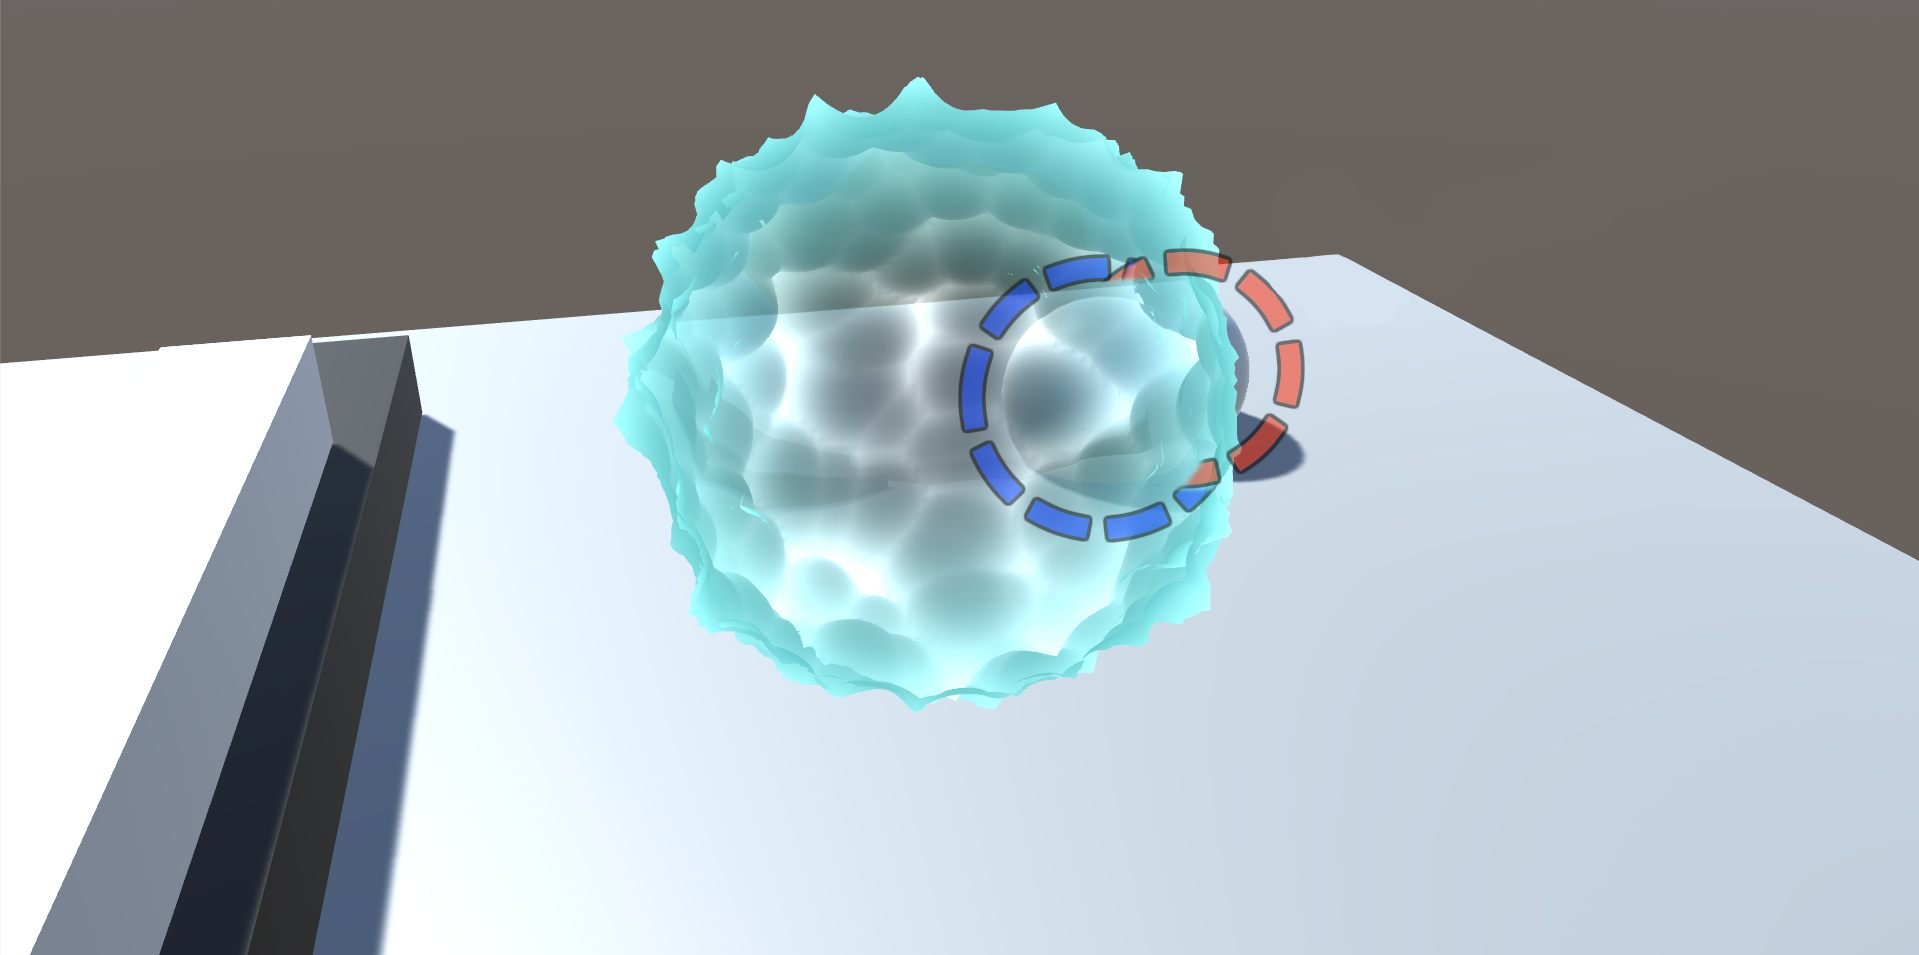
\includegraphics[width=\textwidth]{img/shader_1_guide_v2}
    \caption{Shader - Refraction illustration}
    \label{fig:shader_1}
\end{figure}
\autoref{fig:shader_1} shows a capture of the scene with the shader applied to a sphere. The effect of the Grabpass can be seen as a substitude for refraction, see \secref{sec:refl_refr} \& \secref{sec:grabpass}.\\

The red indicator on the figure shows the original real position of a sphere which is placed behind the object with the shader applied. The blue indicators denote the distortion of the image with the new location of the object being refracted.\\Technically, the shader does not have any transparent properties, instead a Grabpass is used which is discussed in \secref{sec:grabpass}.\\

This gives a better refraction of the object(subjective), compared to when cubemap refractions are used. Since cubemaps require an object to be in a static position in space or constantly update a cubemap image, the grabpass is a faster and more "headache free" alternative.\\


\begin{figure}[H]
    \centering
    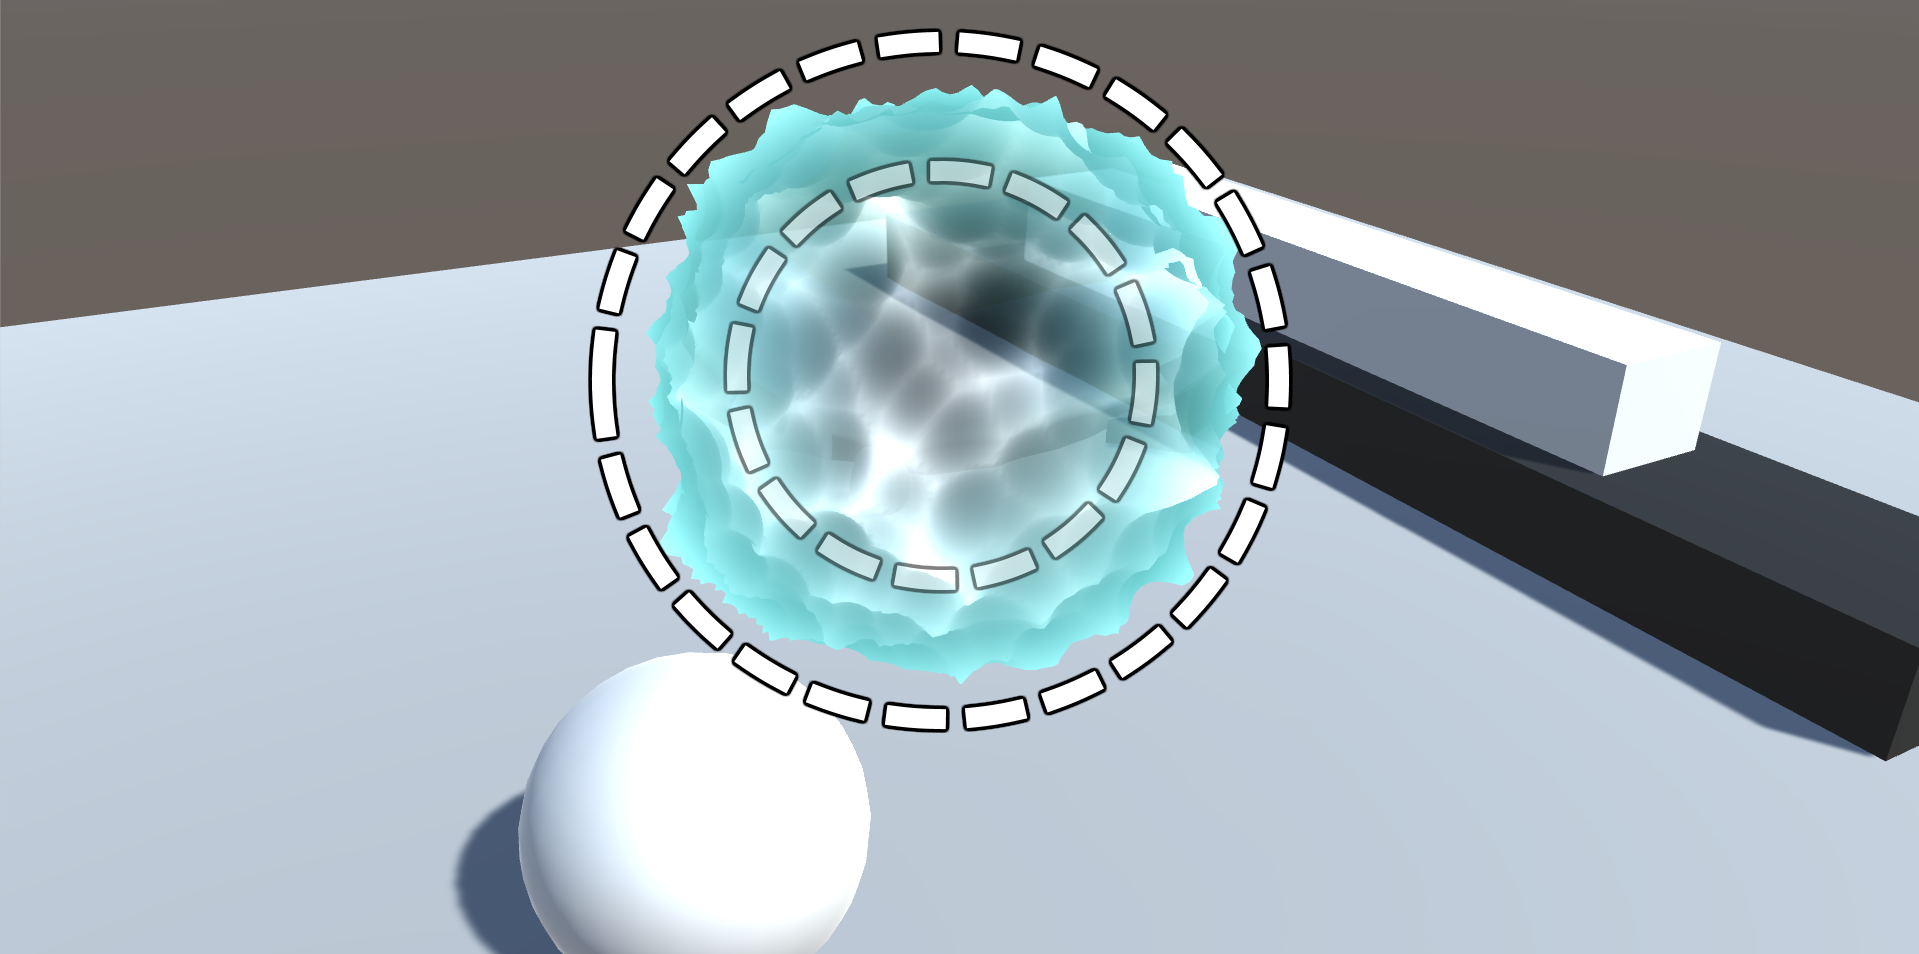
\includegraphics[width=\textwidth]{img/shader_2}
    \caption{Shader, fresnel effect and additive bumpmap}
    \label{fig:shader_2}
\end{figure}
\autoref{fig:shader_2} shows the fresnel effect with some added extra colours from the pre-defined color of the shader and the voronoi bump map colors. Within the markers the fresnel effect should be quite obvious, standing out as a cyan color which is based on a default color input variable. The fresnel effect in this case does not increase or decrease color but tells the shader how much of the grap-pass is shown(refraction) from the other side of the object. The fresnel effect is based on arbitrary values but can be modified in the editor. %CONFIRM THIS
%TODO

\begin{figure}[H]
    \centering
    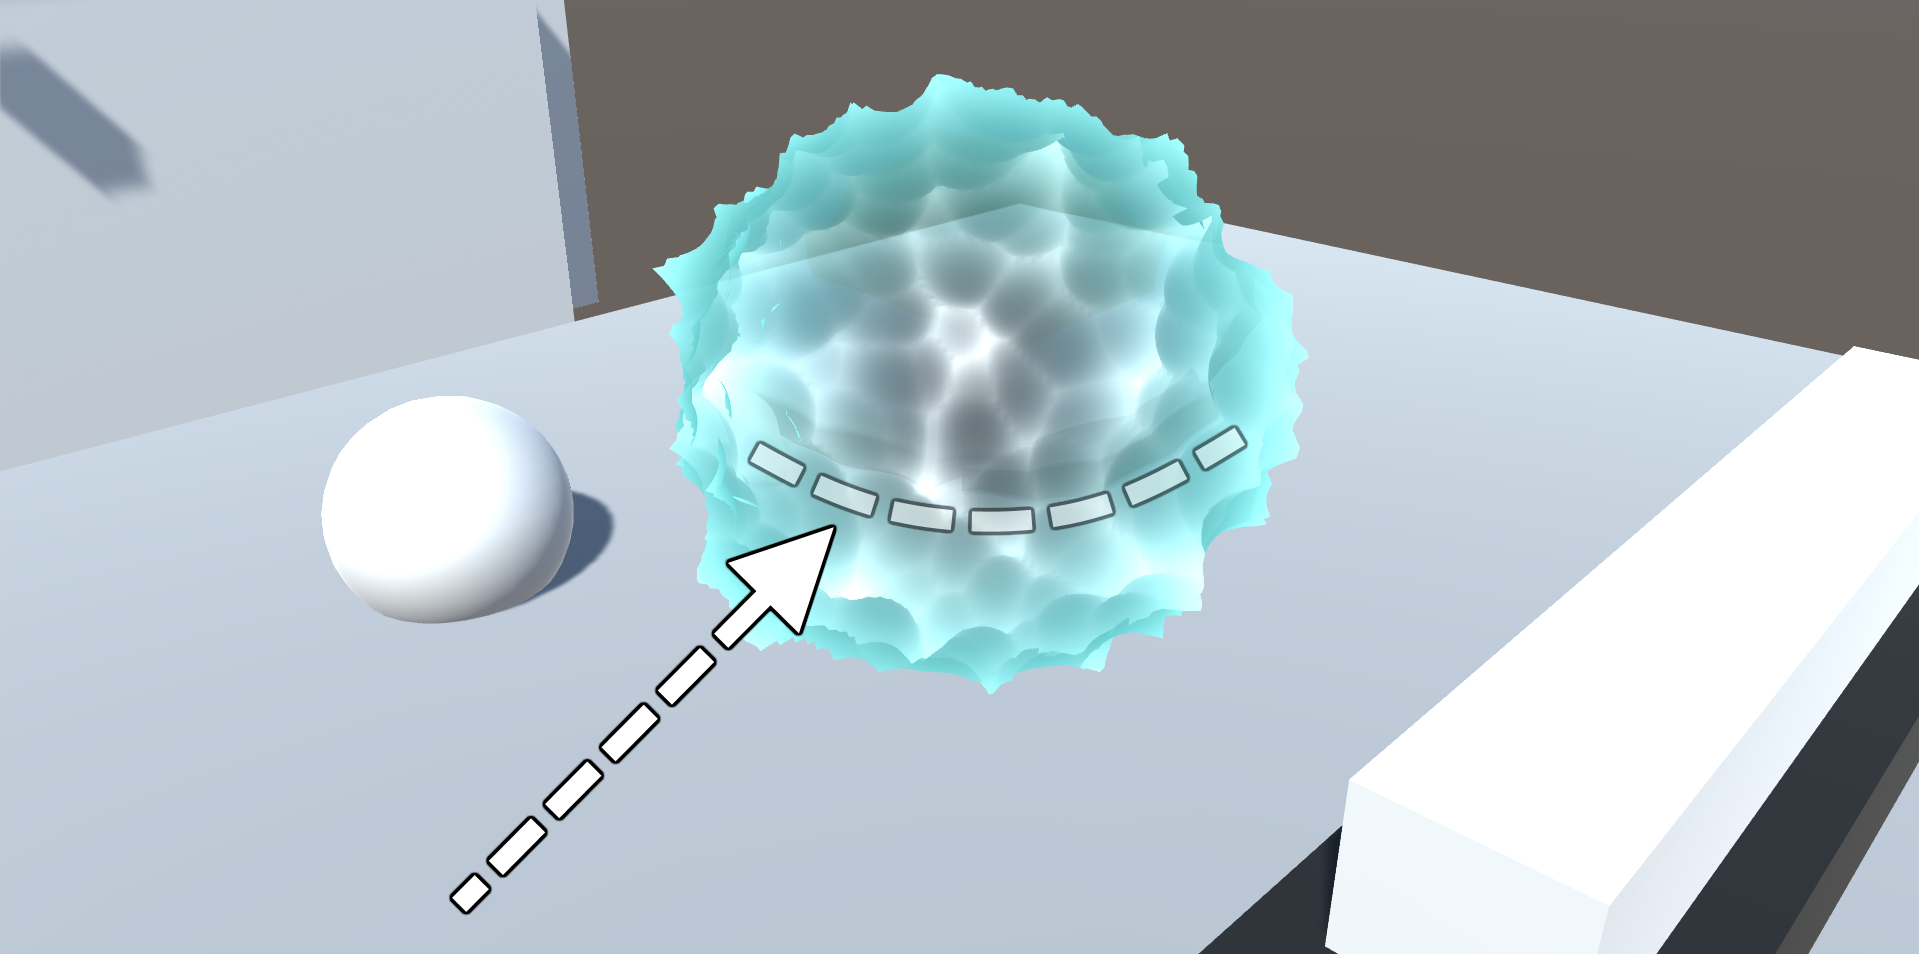
\includegraphics[width=\textwidth]{img/shader_3}
    \caption{Shader}
    \label{fig:shader_3}
\end{figure}
\begin{figure}[H]
    \centering
    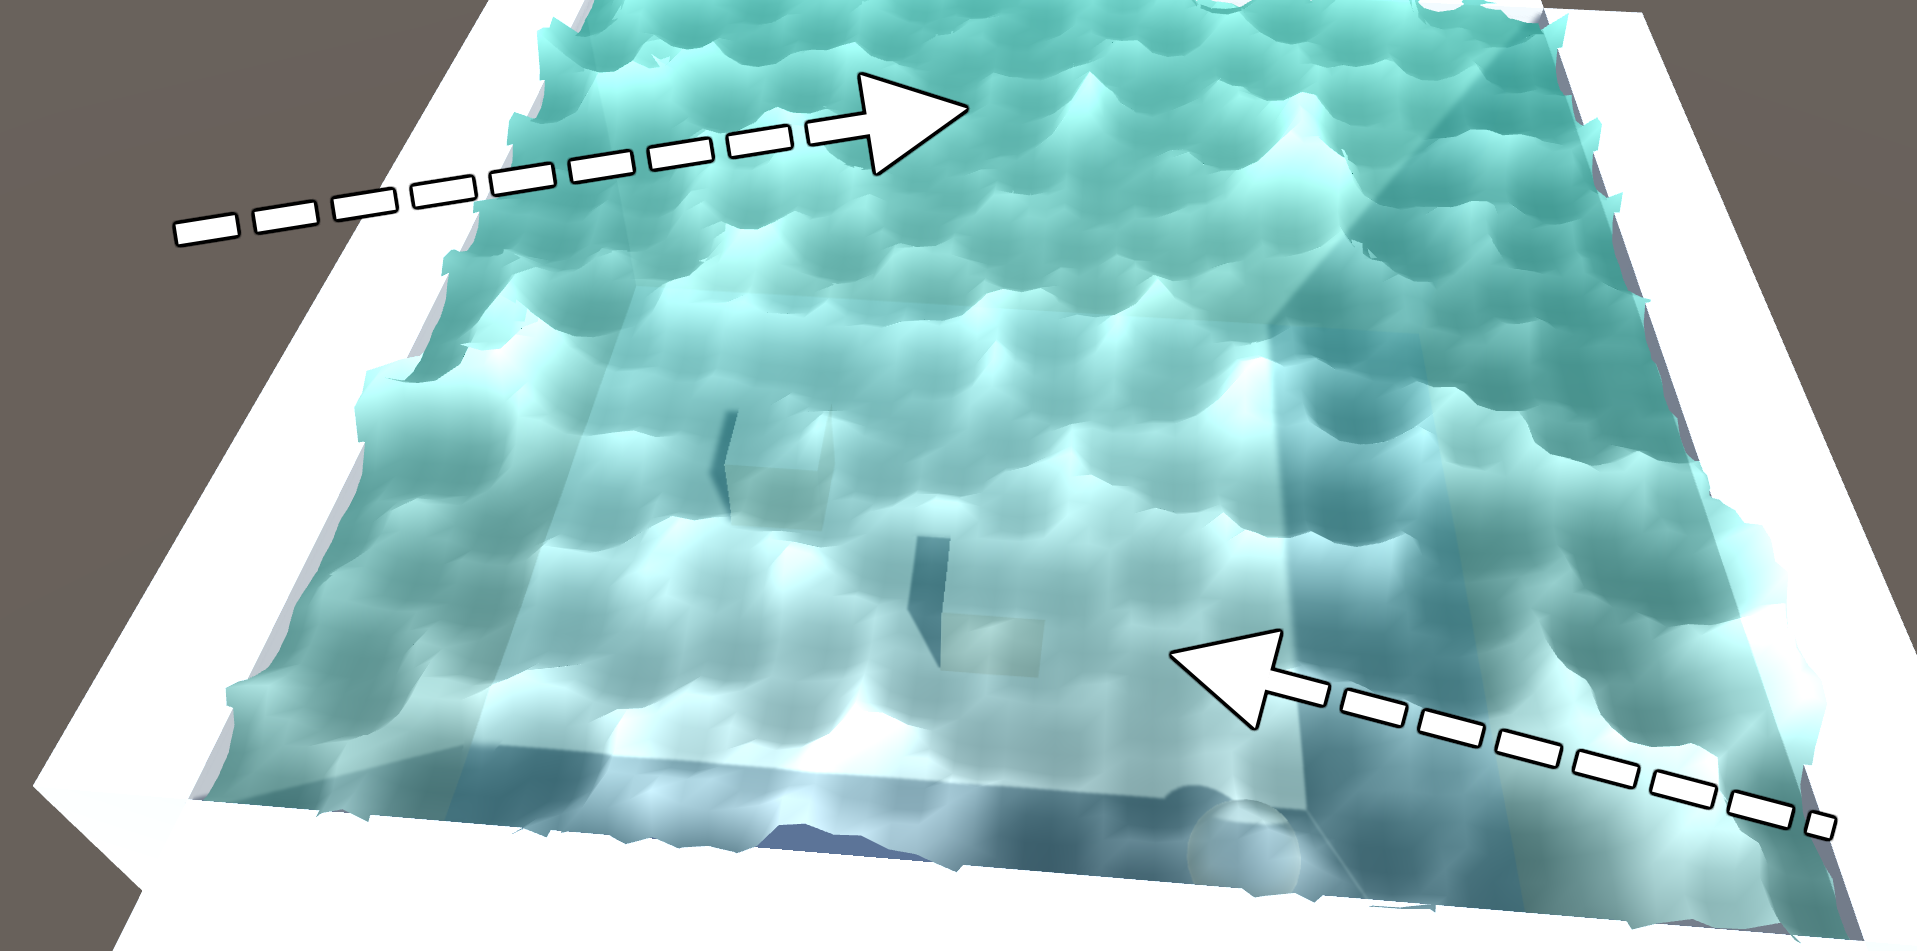
\includegraphics[width=\textwidth]{img/shader_4}
    \caption{Shader}
    \label{fig:shader_4}
\end{figure}

\begin{figure}[H]
    \centering
    \lstinputlisting[firstline=90, lastline=101]{img/voronoi.shader}
    \caption{Voronoi - code implementation in object space}
    \label{fig:voronoi_shader}
\end{figure}
\autoref{fig:voronoi_shader} shows a code snippet from the voronoi implementation. Usually this is used on 2D textures, but since we want to convert it to 3D space we need to do a 3D grid and not a 2D. This is however not needed on a plane or a mesh that which has the same normal vector across the polygons.\\
This code is a very standard or conventional way of implementing voronoi features, besides the additional for-loop on the z axis.\\

Line 4 to 9 is the core of the function, serving to grab the neighbouring grid to later use as an offset. The \texttt{pointt} variable will then hold a random position and have that position modified by time and arbitrary numbers.\\The distance difference will then be calculated and used for colouring the cell or grid square, compared to other points in neighbouring grid cells.

\section{Discussion}
\label{sec:discussion}
I would claim that my approach to a water-shader is more artistic than useful. Usually water-shaders are implemented with a moving bump or normal-map to save frames and achieve a look that better resembles actual waves. My reasoning to go with this approach however, was to try and challenge myself in a more code-heavy implementation (voronoi bump-map), instead of going the conventional route.\\

One problem which I could not overcome without a possible define statement, was that the normals of a plane in Unity would just optimise to one normal, whereas in my 3D program, when I upped the amount of verteces, and thereby the amount of normals I imagined I could affect multiple normals differently, ergo having the shader work both on round and square objects. However Unity( to the best of my knowledge ), optimises this and if multiple normals have the same direction, it changes all the normals into a single normal.

\section{Conclusion}
\label{sec:conclusion}
%TODO
My shader, although arguably could make a performance hit, it has an unconventional implementation, using voronoi as its bump map. Depending on the voronoi greyscale color the shader will then modify the vertex positions based on a formla.\\It then uses fresnel to determine reflectiveness, depending on the camera, like in real-life if a person was to look into a puddle from different angles.


\newpage
\section{Bibliography}
\printbibliography


\end{document}

